\documentclass[11pt,a4paper]{article}

\usepackage[utf8]{inputenc}
\usepackage[T1]{fontenc}
\usepackage[italian]{babel}
\usepackage{lmodern}
\usepackage[a4paper,top=2.3cm,bottom=2.4cm,left=2.3cm,right=2.3cm,headheight=15pt]{geometry}
\usepackage{xcolor}
\usepackage{array}
\usepackage{longtable}
\usepackage{tabularx}
\usepackage{booktabs}
\usepackage{enumitem}
\usepackage{graphicx}
\usepackage{float}
\usepackage{fancyhdr}
\usepackage{titlesec}
\usepackage{microtype}
\usepackage{amssymb}
\usepackage{caption}
\usepackage{listings}
\usepackage{xurl}
\usepackage[hidelinks]{hyperref}
\usepackage{ragged2e}
\usepackage{needspace}

\graphicspath{{img/}}

\pagestyle{fancy}
\fancyhf{}
\lhead{\small TicketSeller}
\rhead{\small Ingegneria del Software}
\cfoot{\thepage}

\setlength{\parindent}{0pt}
\setlength{\parskip}{5pt}
\setlength{\extrarowheight}{2pt}
\renewcommand{\arraystretch}{1.15}
\emergencystretch=3em

\setlist[itemize]{leftmargin=*,itemsep=2pt,topsep=3pt}
\setlist[enumerate]{leftmargin=*,itemsep=2pt,topsep=3pt}

\newcolumntype{Y}{>{\RaggedRight\arraybackslash}X}
\newcolumntype{L}[1]{>{\RaggedRight\arraybackslash}p{#1}}

\captionsetup{font=small,labelfont=bf}

\newcommand{\code}[1]{\texttt{\detokenize{#1}}}

% Diagramma: \diagramma[larghezza]{file}{didascalia}{etichetta}
\newcommand{\diagramma}[4][\textwidth]{%
\begin{figure}[H]
\centering
\includegraphics[width=#1,height=0.80\textheight,keepaspectratio]{#2}
\caption{#3}
\label{#4}
\end{figure}}

\definecolor{codebg}{gray}{0.96}
\lstset{
  language=Python,
  basicstyle=\ttfamily\footnotesize,
  keywordstyle=\bfseries\color{blue!55!black},
  stringstyle=\color{green!40!black},
  commentstyle=\itshape\color{gray},
  backgroundcolor=\color{codebg},
  frame=single, framerule=0pt,
  columns=fullflexible, keepspaces=true,
  breaklines=true, showstringspaces=false,
  xleftmargin=4pt, xrightmargin=4pt, aboveskip=6pt, belowskip=6pt
}

\newcommand{\sectionbreak}{\needspace{0.3\textheight}}
\newcommand{\subsectionbreak}{\needspace{0.15\textheight}}
\titleformat{\section}{\normalfont\Large\bfseries}{\thesection}{0.7em}{}
\titleformat{\subsection}{\normalfont\large\bfseries}{\thesubsection}{0.7em}{}
\titleformat{\subsubsection}{\normalfont\normalsize\bfseries}{\thesubsubsection}{0.7em}{}

\begin{document}

\begin{titlepage}
\centering
\vspace*{0.8cm}

\includegraphics[width=0.28\textwidth]{logo_univpm.png}\par
\vspace{0.9cm}
{\Large\textbf{Università Politecnica delle Marche}\par}
\vspace{0.2cm}
{\large Corso di Ingegneria del Software\par}
\vspace{2.2cm}
{\Huge\bfseries TicketSeller\par}
\vspace{0.4cm}
{\Large Sistema di vendita di biglietti per eventi\par}
\vspace{0.2cm}
{\large Documentazione di progetto\par}
\vfill
\begin{tabular}{@{}ll@{}}
\textbf{Docente:} & Prof. Domenico Ursino \\[2pt]
\textbf{Esercitatore:} & Davide Traini \\[2pt]
\textbf{Studente:} & Kullolli Aaron \\
\end{tabular}
\vspace{1.5cm}

{\large Anno Accademico 2025--2026\par}
\end{titlepage}

\pagenumbering{roman}
\tableofcontents
\newpage
\pagenumbering{arabic}

\section{Descrizione del progetto}
\label{sec:descrizione}

TicketSeller è un programma per vendere biglietti di eventi come concerti, spettacoli teatrali e altri eventi culturali. Lo usano due tipi di persone: i \emph{clienti}, che comprano i biglietti da soli su una postazione self-service chiamata \emph{kiosk}, e i \emph{cassieri}, cioè i dipendenti della biglietteria che gestiscono l'elenco degli eventi.

Per ogni evento si registrano il nome, la data e l'ora, la sala, una descrizione facoltativa, il numero di posti e il prezzo del biglietto. Ogni posto dell'evento ha un suo biglietto, che può essere \emph{disponibile}, \emph{bloccato} (riservato per pochi minuti a un cliente che sta pagando) oppure \emph{venduto}.

Il cliente vede l'elenco degli eventi in programma, ne sceglie uno e vede la mappa dei posti con lo stato e il prezzo di ciascuno. Seleziona i posti liberi che vuole e il programma gli mostra il totale. Poi inserisce nome, e-mail e dati della carta di credito e conferma l'acquisto.

A quel punto il programma controlla che i posti siano ancora liberi e li blocca a nome del cliente, così nessun altro può prenderli. Calcola il totale e chiede il pagamento al servizio della carta di credito (nel progetto il pagamento è simulato). Se il pagamento va a buon fine i biglietti diventano venduti e il cliente riceve un codice che vale come biglietto; se il pagamento non va a buon fine, oppure i dati della carta sono sbagliati, i posti tornano liberi. Un posto non può restare bloccato più di 15 minuti: passato questo tempo torna libero da solo.

Il prezzo può essere calcolato in tre modi: prezzo normale, sconto per i gruppi (sconto in percentuale da un certo numero di biglietti in su) e abbonamento. Un abbonamento ha un codice, vale per alcuni eventi e dà uno sconto: se il cliente inserisce il codice, i biglietti degli eventi compresi nell'abbonamento costano meno, gli altri hanno il prezzo normale.

Il cassiere può aggiungere nuovi eventi, purché in una data futura, modificarli (senza scendere sotto il numero di biglietti già venduti) ed eliminarli, purché nessun biglietto sia stato venduto o sia in fase di pagamento.

I dati vengono salvati sul computer, così restano disponibili anche dopo aver chiuso il programma.

\section{Glossario dei termini}
\label{sec:glossario}

Il glossario spiega i termini che possono creare confusione. Per ognuno è indicato se è un termine del dominio (business) o tecnico e con quali altri nomi compare nel documento o nel programma.

\small
\begin{center}
\begin{tabular}{@{}L{2.9cm}L{7.0cm}L{1.5cm}L{3.0cm}@{}}
\toprule
\textbf{Termine} & \textbf{Descrizione} & \textbf{Tipo} & \textbf{Sinonimi} \\
\midrule
Evento & Spettacolo in una data e in una sala per il quale si vendono biglietti. & Business & Event \\
Catalogo & Insieme degli eventi gestiti dal sistema. & Business & Catalogo eventi \\
Sala & Luogo in cui si svolge l'evento. & Business & Venue \\
Capienza & Numero di posti dell'evento. & Business & Capacity \\
Posto & Singolo posto numerato di un evento. & Business & Seat \\
Mappa dei posti & Elenco dei posti di un evento con stato e prezzo. & Business & Pianta dei posti, seating map \\
Biglietto & Titolo di accesso relativo a un posto di un evento. & Business & Ticket \\
Titolo di accesso & Documento che dà diritto ad accedere a uno o più eventi: biglietto o abbonamento. & Business & Voucher \\
Abbonamento & Titolo di accesso, identificato da un codice, che copre un insieme di eventi e prevede uno sconto sui relativi biglietti. & Business & Subscription \\
Prezzo base & Prezzo pieno di un biglietto dell'evento. & Business & Base price \\
Politica di prezzo & Regola con cui si calcola il totale: standard, gruppo o abbonamento. & Business & Strategia di prezzo \\
Prenotazione temporanea & Blocco di uno o più posti a nome di un cliente durante l'acquisto, per al massimo 15 minuti. & Business & Blocco, posto bloccato, locked \\
Acquisto & Blocco dei posti, calcolo del totale, pagamento e conferma o annullamento. & Business & Checkout, vendita \\
Cliente & Persona che acquista biglietti dal kiosk. & Business & Customer \\
Cassiere & Dipendente della biglietteria che gestisce il catalogo. & Business & Clerk \\
Utente & Chi usa il sistema (cliente o cassiere). & Tecnico & User \\
Kiosk & Postazione self-service del cliente. & Tecnico & KioskInterface \\
Postazione cassiere & Postazione per la gestione del catalogo. & Tecnico & ClerkInterface \\
Servizio di pagamento & Sistema esterno che autorizza o rifiuta l'addebito sulla carta; nel prototipo è simulato. & Tecnico & CreditCardCharges \\
Codice di transazione & Identificativo restituito per un pagamento approvato; è mostrato al cliente come titolo di accesso. & Tecnico & Transaction id \\
Archivio dati & File sul computer in cui sono salvati eventi, biglietti e abbonamenti. & Tecnico & Persistenza, database \\
\bottomrule
\end{tabular}
\end{center}
\normalsize

\section{Analisi dei requisiti}
\label{sec:requisiti}

I requisiti funzionali dicono cosa deve fare il sistema; quelli non funzionali indicano vincoli e qualità che deve rispettare. Ogni requisito ha un codice e un nome, gli stessi del diagramma, ed è scritto in modo da poter verificare se è rispettato. I requisiti funzionali sono divisi in due aree: gestione degli eventi e gestione delle vendite.

\diagramma[0.95\textwidth]{Analisi_dei_Requisiti.png}{Diagramma dei requisiti}{fig:requisiti}

\subsection{Requisiti funzionali}

\textbf{Area: Gestione Eventi}

\begin{description}[style=nextline,leftmargin=0.6cm,itemsep=3pt]
\item[RF1 -- Mostra eventi futuri] Quando il cliente apre o aggiorna la schermata del kiosk, il sistema dovrà mostrare l'elenco degli eventi con data futura, in ordine cronologico.
\item[RF2 -- Mostra mappa posti] Quando il cliente seleziona un evento, il sistema dovrà mostrare la mappa dei posti dell'evento con lo stato (disponibile, bloccato, venduto) e il prezzo di ciascun posto, consentendo di selezionare solo i posti disponibili.
\item[RF10 -- Cassiere crea evento futuro] Quando il cassiere inserisce i dati di un nuovo evento (identificativo, nome, data, capienza, prezzo base, sala), il sistema dovrà memorizzare l'evento nel catalogo e generarne la mappa dei posti; dovrà rifiutare eventi con data passata, nome vuoto, capienza non positiva, prezzo negativo o identificativo già esistente.
\item[RF11 -- Cassiere aggiorna evento futuro] Quando il cassiere modifica i dati di un evento esistente, il sistema dovrà aggiornare l'evento, la sua mappa dei posti e il prezzo dei posti ancora disponibili; dovrà rifiutare date passate e capienze inferiori al numero di biglietti già venduti.
\item[RF12 -- Cassiere elimina evento futuro] Quando il cassiere richiede l'eliminazione di un evento senza biglietti venduti o bloccati, il sistema dovrà eliminare l'evento e i relativi posti dal catalogo; altrimenti dovrà rifiutare l'operazione.
\end{description}

\textbf{Area: Gestione Vendite}

\begin{description}[style=nextline,leftmargin=0.6cm,itemsep=3pt]
\item[RF3 -- Prenotazione temporanea posti] Quando il cliente conferma l'acquisto dei posti selezionati, il sistema dovrà verificare che tutti i posti esistano, siano distinti e siano disponibili e, in caso positivo, bloccarli temporaneamente a nome del cliente; se almeno un posto non è disponibile dovrà rifiutare l'intera richiesta.
\item[RF4 -- Inserimento dati carta di credito] Il sistema dovrà consentire al cliente di inserire i dati della carta di credito (titolare, numero, mese e anno di scadenza, CVV) e dovrà rifiutare dati formalmente non validi: titolare vuoto, numero non numerico o con meno di 12 cifre, mese non compreso tra 1 e 12, carta scaduta, CVV diverso da 3 o 4 cifre.
\item[RF5 -- Calcolo totale ordine] Quando il cliente seleziona uno o più posti, il sistema dovrà calcolare il totale dell'ordine applicando la politica di prezzo in vigore e mostrarlo al cliente; lo stesso calcolo dovrà essere ripetuto al momento dell'acquisto sui posti bloccati.
\item[RF6 -- Invio pagamento a servizio esterno] Quando i posti sono stati bloccati e il totale è stato calcolato, il sistema dovrà inviare al servizio di pagamento esterno i dati della carta e l'importo totale.
\item[RF7 -- Conferma vendita e rilascio titoli] Quando il servizio di pagamento approva il pagamento, il sistema dovrà registrare i biglietti bloccati come venduti al cliente e mostrargli il codice della transazione, che costituisce il titolo di accesso.
\item[RF8 -- Annulla prenotazione se rifiutato] Quando il pagamento è rifiutato dal servizio di pagamento o non può essere eseguito perché i dati della carta non sono validi, il sistema dovrà annullare il blocco dei posti, rendendoli di nuovo disponibili, e informare il cliente dell'esito.
\item[RF9 -- Rilascia biglietti a timeout scaduto] Quando un posto rimane bloccato per 15 minuti o più senza che l'acquisto sia stato concluso, il sistema dovrà renderlo nuovamente disponibile entro un minuto, e comunque prima di mostrare la mappa dei posti o di bloccare posti dello stesso evento.
\item[RF13 -- Applica abbonamento al totale] Quando il cliente indica il codice di un abbonamento durante l'acquisto, il sistema dovrà applicare lo sconto dell'abbonamento ai biglietti degli eventi coperti e il prezzo pieno ai biglietti degli altri eventi; un codice inesistente dovrà essere rifiutato.
\end{description}

\subsection{Requisiti non funzionali}

\begin{description}[style=nextline,leftmargin=0.6cm,itemsep=3pt]
\item[RNF1 -- Implementazione in Python 3] Vincolo: il sistema dovrà essere realizzato in linguaggio Python 3, versione 3.11 o successiva.
\item[RNF2 -- Fornire interfaccia GUI desktop con PyQt] Vincolo: il sistema dovrà fornire due interfacce grafiche desktop realizzate con PyQt6, una per il cliente (kiosk) e una per il cassiere.
\item[RNF3 -- Prevenzione doppie prenotazioni (accessi concorrenti)] Il sistema non dovrà mai bloccare o vendere lo stesso posto a due clienti: se più richieste sullo stesso posto arrivano nello stesso momento, al più una dovrà andare a buon fine.
\item[RNF4 -- Precisione decimale esatta degli importi] Tutti gli importi monetari dovranno essere rappresentati e calcolati in aritmetica decimale esatta, con risultato arrotondato al centesimo di euro (ad esempio $0{,}10 + 0{,}20 = 0{,}30$ e $5{,}025 \rightarrow 5{,}03$).
\item[RNF5 -- Persistenza astratta e separata dalla logica di business] I dati di eventi, biglietti e abbonamenti dovranno essere conservati tra due esecuzioni del programma e la logica applicativa dovrà accedervi solo tramite interfacce dedicate (DAO), così che il modo di salvare i dati (oggi un file) possa essere cambiato senza modificarla.
\item[RNF6 -- Testing unitario isolato] Le classi del modello, del controller e della persistenza dovranno poter essere verificate con test PyUnit automatici eseguibili senza interfaccia grafica e senza il servizio di pagamento reale.
\item[RNF7 -- Timeout massimo della prenotazione temporanea] La durata massima di una prenotazione temporanea dovrà essere di 15 minuti.
\end{description}

\section{Casi d'uso}
\label{sec:casiuso}

\subsection{Attori}

\diagramma[0.42\textwidth]{Attori.png}{Attori del sistema}{fig:attori}

\begin{tabularx}{\textwidth}{@{}L{3.6cm}Y@{}}
\toprule
\textbf{Attore} & \textbf{Descrizione} \\
\midrule
Cliente & Persona che consulta gli eventi e acquista biglietti dal kiosk. \\
Cassiere & Dipendente della biglietteria che gestisce il catalogo degli eventi. \\
Servizio di pagamento & Sistema esterno che autorizza o rifiuta l'addebito sulla carta (attore secondario). \\
Tempo & Attore non umano che rappresenta il trascorrere del tempo e avvia l'annullamento delle prenotazioni scadute. \\
\bottomrule
\end{tabularx}

Il sistema stesso e il suo archivio dati non sono attori, perché fanno parte del sistema.

\subsection{Diagramma dei casi d'uso}

\diagramma[0.9\textwidth]{Ticketseller.png}{Diagramma dei casi d'uso}{fig:casiduso}

UC2 e UC3 \emph{includono} UC6: prima di mostrare la mappa e prima di bloccare i posti il sistema libera sempre i posti bloccati da troppo tempo, così il cliente vede la situazione aggiornata. UC4 \emph{estende} UC3: viene eseguito solo se il cliente inserisce un abbonamento. L'attore Tempo avvia UC6; il Servizio di pagamento partecipa all'acquisto.

\subsection{Schede dei casi d'uso}


\begin{center}
\small
\begin{tabular}{|p{0.86\textwidth}|}
\hline
\textbf{Caso d'uso: Consultazione eventi} \\ \hline
\textbf{ID:} UC1 \\ \hline
\textbf{Breve descrizione:}\newline Il sistema mostra al cliente gli eventi futuri in programma. \\ \hline
\textbf{Attori primari:}\newline Cliente \\ \hline
\textbf{Attori secondari:}\newline Nessuno \\ \hline
\textbf{Precondizioni:}\newline L'applicazione è avviata in modalità kiosk. \\ \hline
\textbf{Sequenza degli eventi principale:}\newline 1.~Il caso d'uso inizia quando il Cliente apre la schermata del kiosk o seleziona ``Refresh''.\newline
2.~Il sistema recupera dal catalogo gli eventi con data futura.\newline
3.~Il sistema mostra gli eventi in ordine cronologico. \\ \hline
\textbf{Postcondizioni:}\newline Il Cliente visualizza l'elenco degli eventi futuri. \\ \hline
\textbf{Sequenza degli eventi alternativa:}\newline 2a.~Se non ci sono eventi futuri, l'elenco è vuoto. \\ \hline
\end{tabular}
\end{center}

\begin{center}
\small
\begin{tabular}{|p{0.86\textwidth}|}
\hline
\textbf{Caso d'uso: Selezione posti} \\ \hline
\textbf{ID:} UC2 \\ \hline
\textbf{Breve descrizione:}\newline Il cliente visualizza la mappa dei posti di un evento e seleziona i posti; il sistema mostra il totale. \\ \hline
\textbf{Attori primari:}\newline Cliente \\ \hline
\textbf{Attori secondari:}\newline Nessuno \\ \hline
\textbf{Precondizioni:}\newline Il Cliente visualizza l'elenco degli eventi futuri (UC1). \\ \hline
\textbf{Sequenza degli eventi principale:}\newline 1.~Il caso d'uso inizia quando il Cliente seleziona un evento.\newline
2.~include(Annullamento automatico).\newline
3.~Il sistema mostra la mappa dei posti con stato e prezzo; i posti non disponibili non sono selezionabili.\newline
4.~Il Cliente seleziona uno o più posti disponibili.\newline
5.~Il sistema calcola e mostra il totale. \\ \hline
\textbf{Postcondizioni:}\newline I posti sono selezionati e il totale è visualizzato; nessun posto è ancora bloccato. \\ \hline
\textbf{Sequenza degli eventi alternativa:}\newline Nessuna. \\ \hline
\end{tabular}
\end{center}

\begin{center}
\small
\begin{tabular}{|p{0.86\textwidth}|}
\hline
\textbf{Caso d'uso: Acquisto titolo di accesso} \\ \hline
\textbf{ID:} UC3 \\ \hline
\textbf{Breve descrizione:}\newline Il cliente acquista i posti selezionati: il sistema li blocca, richiede il pagamento e conferma la vendita oppure annulla il blocco. \\ \hline
\textbf{Attori primari:}\newline Cliente \\ \hline
\textbf{Attori secondari:}\newline Servizio di pagamento \\ \hline
\textbf{Precondizioni:}\newline Il Cliente ha selezionato almeno un posto di un evento futuro (UC2). \\ \hline
\textbf{Sequenza degli eventi principale:}\newline 1.~Il caso d'uso inizia quando il Cliente inserisce nome, e-mail e dati della carta e seleziona ``Buy Selected Seats''.\newline
2.~include(Annullamento automatico).\newline
3.~\textbf{if} i posti non sono distinti, non esistono o almeno uno non è disponibile\newline
\hspace*{1em}3.1.~il sistema mostra un messaggio di errore e il caso d'uso termina.\newline
4.~Il sistema blocca i posti a nome del Cliente.\newline
5.~Il sistema calcola il totale con la politica di prezzo in vigore.\newline
\hspace*{1em}punto di estensione: \emph{applicazione abbonamento}\newline
6.~Il sistema invia dati della carta e totale al Servizio di pagamento.\newline
7.~\textbf{if} il pagamento è approvato\newline
\hspace*{1em}7.1.~il sistema registra i biglietti come venduti al Cliente;\newline
\hspace*{1em}7.2.~il sistema mostra il codice della transazione.\newline
8.~\textbf{else}\newline
\hspace*{1em}8.1.~il sistema annulla il blocco dei posti e mostra l'esito negativo.\newline
9.~Il sistema aggiorna la mappa dei posti. \\ \hline
\textbf{Postcondizioni:}\newline I biglietti sono venduti al Cliente, oppure i posti sono di nuovo disponibili. \\ \hline
\textbf{Sequenza degli eventi alternativa:}\newline 6a.~Se i dati della carta non sono validi, il sistema annulla il blocco dei posti e mostra un messaggio di errore. \\ \hline
\end{tabular}
\end{center}

\begin{center}
\small
\begin{tabular}{|p{0.86\textwidth}|}
\hline
\textbf{Caso d'uso di estensione: Utilizzo abbonamento} \\ \hline
\textbf{ID:} UC4 \\ \hline
\textbf{Breve descrizione:}\newline Segmento 1: il cliente indica il codice di un abbonamento e il sistema sconta i biglietti degli eventi coperti. \\ \hline
\textbf{Attori primari:}\newline Cliente \\ \hline
\textbf{Attori secondari:}\newline Nessuno \\ \hline
\textbf{Precondizioni del segmento 1:}\newline È in corso un acquisto (UC3) al punto di estensione \emph{applicazione abbonamento} e il Cliente ha inserito un codice abbonamento. \\ \hline
\textbf{Sequenza degli eventi del segmento 1:}\newline 1.~Il sistema cerca l'abbonamento con il codice indicato.\newline
2.~\textbf{for each} biglietto dell'ordine\newline
\hspace*{1em}2.1.~\textbf{if} l'evento è coperto, il sistema applica lo sconto dell'abbonamento;\newline
\hspace*{1em}2.2.~\textbf{else} il sistema applica il prezzo pieno.\newline
3.~Il sistema restituisce a UC3 il totale arrotondato al centesimo. \\ \hline
\textbf{Postcondizioni del segmento 1:}\newline Il totale tiene conto dell'abbonamento. \\ \hline
\textbf{Sequenza degli eventi alternativa:}\newline 1a.~Se il codice non esiste, il sistema mostra un messaggio di errore e il totale resta invariato. \\ \hline
\end{tabular}
\end{center}

\begin{center}
\small
\begin{tabular}{|p{0.86\textwidth}|}
\hline
\textbf{Caso d'uso: Gestione catalogo eventi} \\ \hline
\textbf{ID:} UC5 \\ \hline
\textbf{Breve descrizione:}\newline Il cassiere crea, modifica o elimina un evento del catalogo. \\ \hline
\textbf{Attori primari:}\newline Cassiere \\ \hline
\textbf{Attori secondari:}\newline Nessuno \\ \hline
\textbf{Precondizioni:}\newline L'applicazione è avviata in modalità cassiere. \\ \hline
\textbf{Sequenza degli eventi principale:}\newline 1.~Il caso d'uso inizia quando il Cassiere vuole effettuare un'operazione sul catalogo.\newline
2.~\textbf{if} il Cassiere vuole creare un evento\newline
\hspace*{1em}2.1.~il Cassiere inserisce identificativo, nome, data, capienza, prezzo e sala;\newline
\hspace*{1em}2.2.~\textbf{if} il cassiere non è valido, la data è passata o i dati non sono validi, il sistema mostra un errore;\newline
\hspace*{1em}2.3.~\textbf{else} il sistema memorizza l'evento e ne genera la mappa dei posti.\newline
3.~\textbf{else if} il Cassiere vuole modificare un evento\newline
\hspace*{1em}3.1.~il Cassiere seleziona l'evento e ne modifica i dati;\newline
\hspace*{1em}3.2.~\textbf{if} i controlli non sono superati (cassiere, data, capienza minore dei venduti), il sistema mostra un errore;\newline
\hspace*{1em}3.3.~\textbf{else} il sistema aggiorna l'evento e la mappa dei posti.\newline
4.~\textbf{else if} il Cassiere vuole eliminare un evento\newline
\hspace*{1em}4.1.~\textbf{if} il cassiere non è valido o l'evento ha biglietti venduti o bloccati, il sistema mostra un errore;\newline
\hspace*{1em}4.2.~\textbf{else} il sistema elimina l'evento e i suoi posti.\newline
5.~Il sistema aggiorna l'elenco degli eventi. \\ \hline
\textbf{Postcondizioni:}\newline Il catalogo riflette l'operazione richiesta, oppure è invariato e il Cassiere ha ricevuto un messaggio di errore. \\ \hline
\textbf{Sequenza degli eventi alternativa:}\newline Nessuna. \\ \hline
\end{tabular}
\end{center}

\begin{center}
\small
\begin{tabular}{|p{0.86\textwidth}|}
\hline
\textbf{Caso d'uso: Annullamento automatico} \\ \hline
\textbf{ID:} UC6 \\ \hline
\textbf{Breve descrizione:}\newline Il sistema annulla le prenotazioni temporanee che hanno superato i 15 minuti. \\ \hline
\textbf{Attori primari:}\newline Tempo \\ \hline
\textbf{Attori secondari:}\newline Nessuno \\ \hline
\textbf{Precondizioni:}\newline Nessuna. \\ \hline
\textbf{Sequenza degli eventi principale:}\newline 1.~Il caso d'uso inizia ogni minuto (attore Tempo) oppure quando è incluso da UC2 o UC3.\newline
2.~Il sistema acquisisce data e ora correnti.\newline
3.~\textbf{for each} biglietto\newline
\hspace*{1em}3.1.~\textbf{if} il biglietto è bloccato da almeno 15 minuti, il sistema annulla il blocco.\newline
4.~\textbf{if} almeno un biglietto è stato rilasciato, il sistema salva i biglietti aggiornati. \\ \hline
\textbf{Postcondizioni:}\newline Nessun biglietto risulta bloccato da 15 minuti o più. \\ \hline
\textbf{Sequenza degli eventi alternativa:}\newline Nessuna. \\ \hline
\end{tabular}
\end{center}

\subsection{Matrice di mapping}
\label{sec:matrice}

La matrice indica quali requisiti funzionali sono realizzati da ciascun caso d'uso: serve a controllare che ogni requisito sia coperto da almeno uno scenario.

\begin{table}[H]
\centering
\small
\setlength{\tabcolsep}{4pt}
\renewcommand{\arraystretch}{1.5}
\begin{tabular}{|l|c|c|c|c|c|c|c|c|c|c|c|c|c|}
\hline
 & \textbf{RF1} & \textbf{RF2} & \textbf{RF3} & \textbf{RF4} & \textbf{RF5} & \textbf{RF6} & \textbf{RF7} & \textbf{RF8} & \textbf{RF9} & \textbf{RF10} & \textbf{RF11} & \textbf{RF12} & \textbf{RF13} \\
\hline
\textbf{UC1} & $\checkmark$ &  &  &  &  &  &  &  &  &  &  &  &  \\ \hline
\textbf{UC2} &  & $\checkmark$ &  &  & $\checkmark$ &  &  &  & $\checkmark$ &  &  &  &  \\ \hline
\textbf{UC3} &  &  & $\checkmark$ & $\checkmark$ & $\checkmark$ & $\checkmark$ & $\checkmark$ & $\checkmark$ & $\checkmark$ &  &  &  &  \\ \hline
\textbf{UC4} &  &  &  &  & $\checkmark$ &  &  &  &  &  &  &  & $\checkmark$ \\ \hline
\textbf{UC5} &  &  &  &  &  &  &  &  &  & $\checkmark$ & $\checkmark$ & $\checkmark$ &  \\ \hline
\textbf{UC6} &  &  &  &  &  &  &  &  & $\checkmark$ &  &  &  &  \\ \hline
\end{tabular}
\caption{Matrice di mapping casi d'uso -- requisiti funzionali (UC1 Consultazione eventi, UC2 Selezione posti, UC3 Acquisto titolo di accesso, UC4 Utilizzo abbonamento, UC5 Gestione catalogo eventi, UC6 Annullamento automatico)}
\label{tab:matrice}
\end{table}

\section{Analisi}
\label{sec:analisi}

\subsection{Package di analisi}

\diagramma[0.85\textwidth]{PKG_-_Analisi_e_progettazione.png}{Package di analisi}{fig:pkg}

A livello di analisi il sistema è diviso in tre package: \textbf{GestioneEventi} (l'evento e il catalogo), \textbf{GestioneUtenti} (clienti e cassieri) e \textbf{GestioneVendite} (biglietti, abbonamenti e titoli di accesso). GestioneVendite usa gli altri due, perché ogni biglietto si riferisce a un evento e appartiene, se bloccato o venduto, a un cliente.

\subsection{Classi di analisi}

Per ogni package si riporta il diagramma delle classi con gli attributi tipizzati e le associazioni con molteplicità; a questo livello non si indicano le operazioni.

\subsubsection*{GestioneEventi}
\diagramma[0.32\textwidth]{GestioneEventi.png}{Classi di analisi: GestioneEventi}{fig:ca-eventi}

\subsubsection*{GestioneUtenti}
\diagramma[0.75\textwidth]{GestioneUtenti.png}{Classi di analisi: GestioneUtenti}{fig:ca-utenti}
Cliente e cassiere sono specializzazioni di \code{User}; il cassiere ha in più il codice dipendente.

\subsubsection*{GestioneVendite}
\diagramma[0.85\textwidth]{GestioneVendite.png}{Classi di analisi: GestioneVendite}{fig:ca-vendite}
Biglietto e abbonamento sono due tipi di titolo di accesso (\code{Voucher}). Un evento ha uno o più biglietti, uno per posto; un biglietto può appartenere a un cliente; un abbonamento copre zero o più eventi.

\subsection{Diagrammi di sequenza}
\label{sec:sequenza}

Per ogni scenario si riporta un diagramma di sequenza. I messaggi corrispondono ai metodi reali del codice; i messaggi di ritorno sono tratteggiati. L'annullamento delle prenotazioni scadute, incluso da UC2 e UC3, è richiamato con un frammento \texttt{ref} che rimanda al diagramma di UC6.

\subsubsection{UC1 -- Consultazione eventi}
\diagramma[0.6\textwidth]{UC1_-_Consultazione_eventi.png}{Sequenza UC1 -- Consultazione eventi}{fig:sd1}
La vista chiede al controller \code{search_future_events()}, che delega al DAO \code{find_future_events()}; l'elenco ottenuto è mostrato al cliente.

\subsubsection{UC2 -- Selezione posti}
\diagramma[0.6\textwidth]{UC2_-_Selezione_posti.png}{Sequenza UC2 -- Selezione posti}{fig:sd2}
Alla scelta dell'evento il controller esegue prima l'annullamento delle prenotazioni scadute (\texttt{ref} UC6), poi legge i biglietti dell'evento. Quando il cliente seleziona i posti, la vista chiede il totale con \code{calculate_total(tickets, subscription)} e lo mostra.

\subsubsection{UC3 -- Acquisto titolo di accesso}
\begin{figure}[H]
\centering
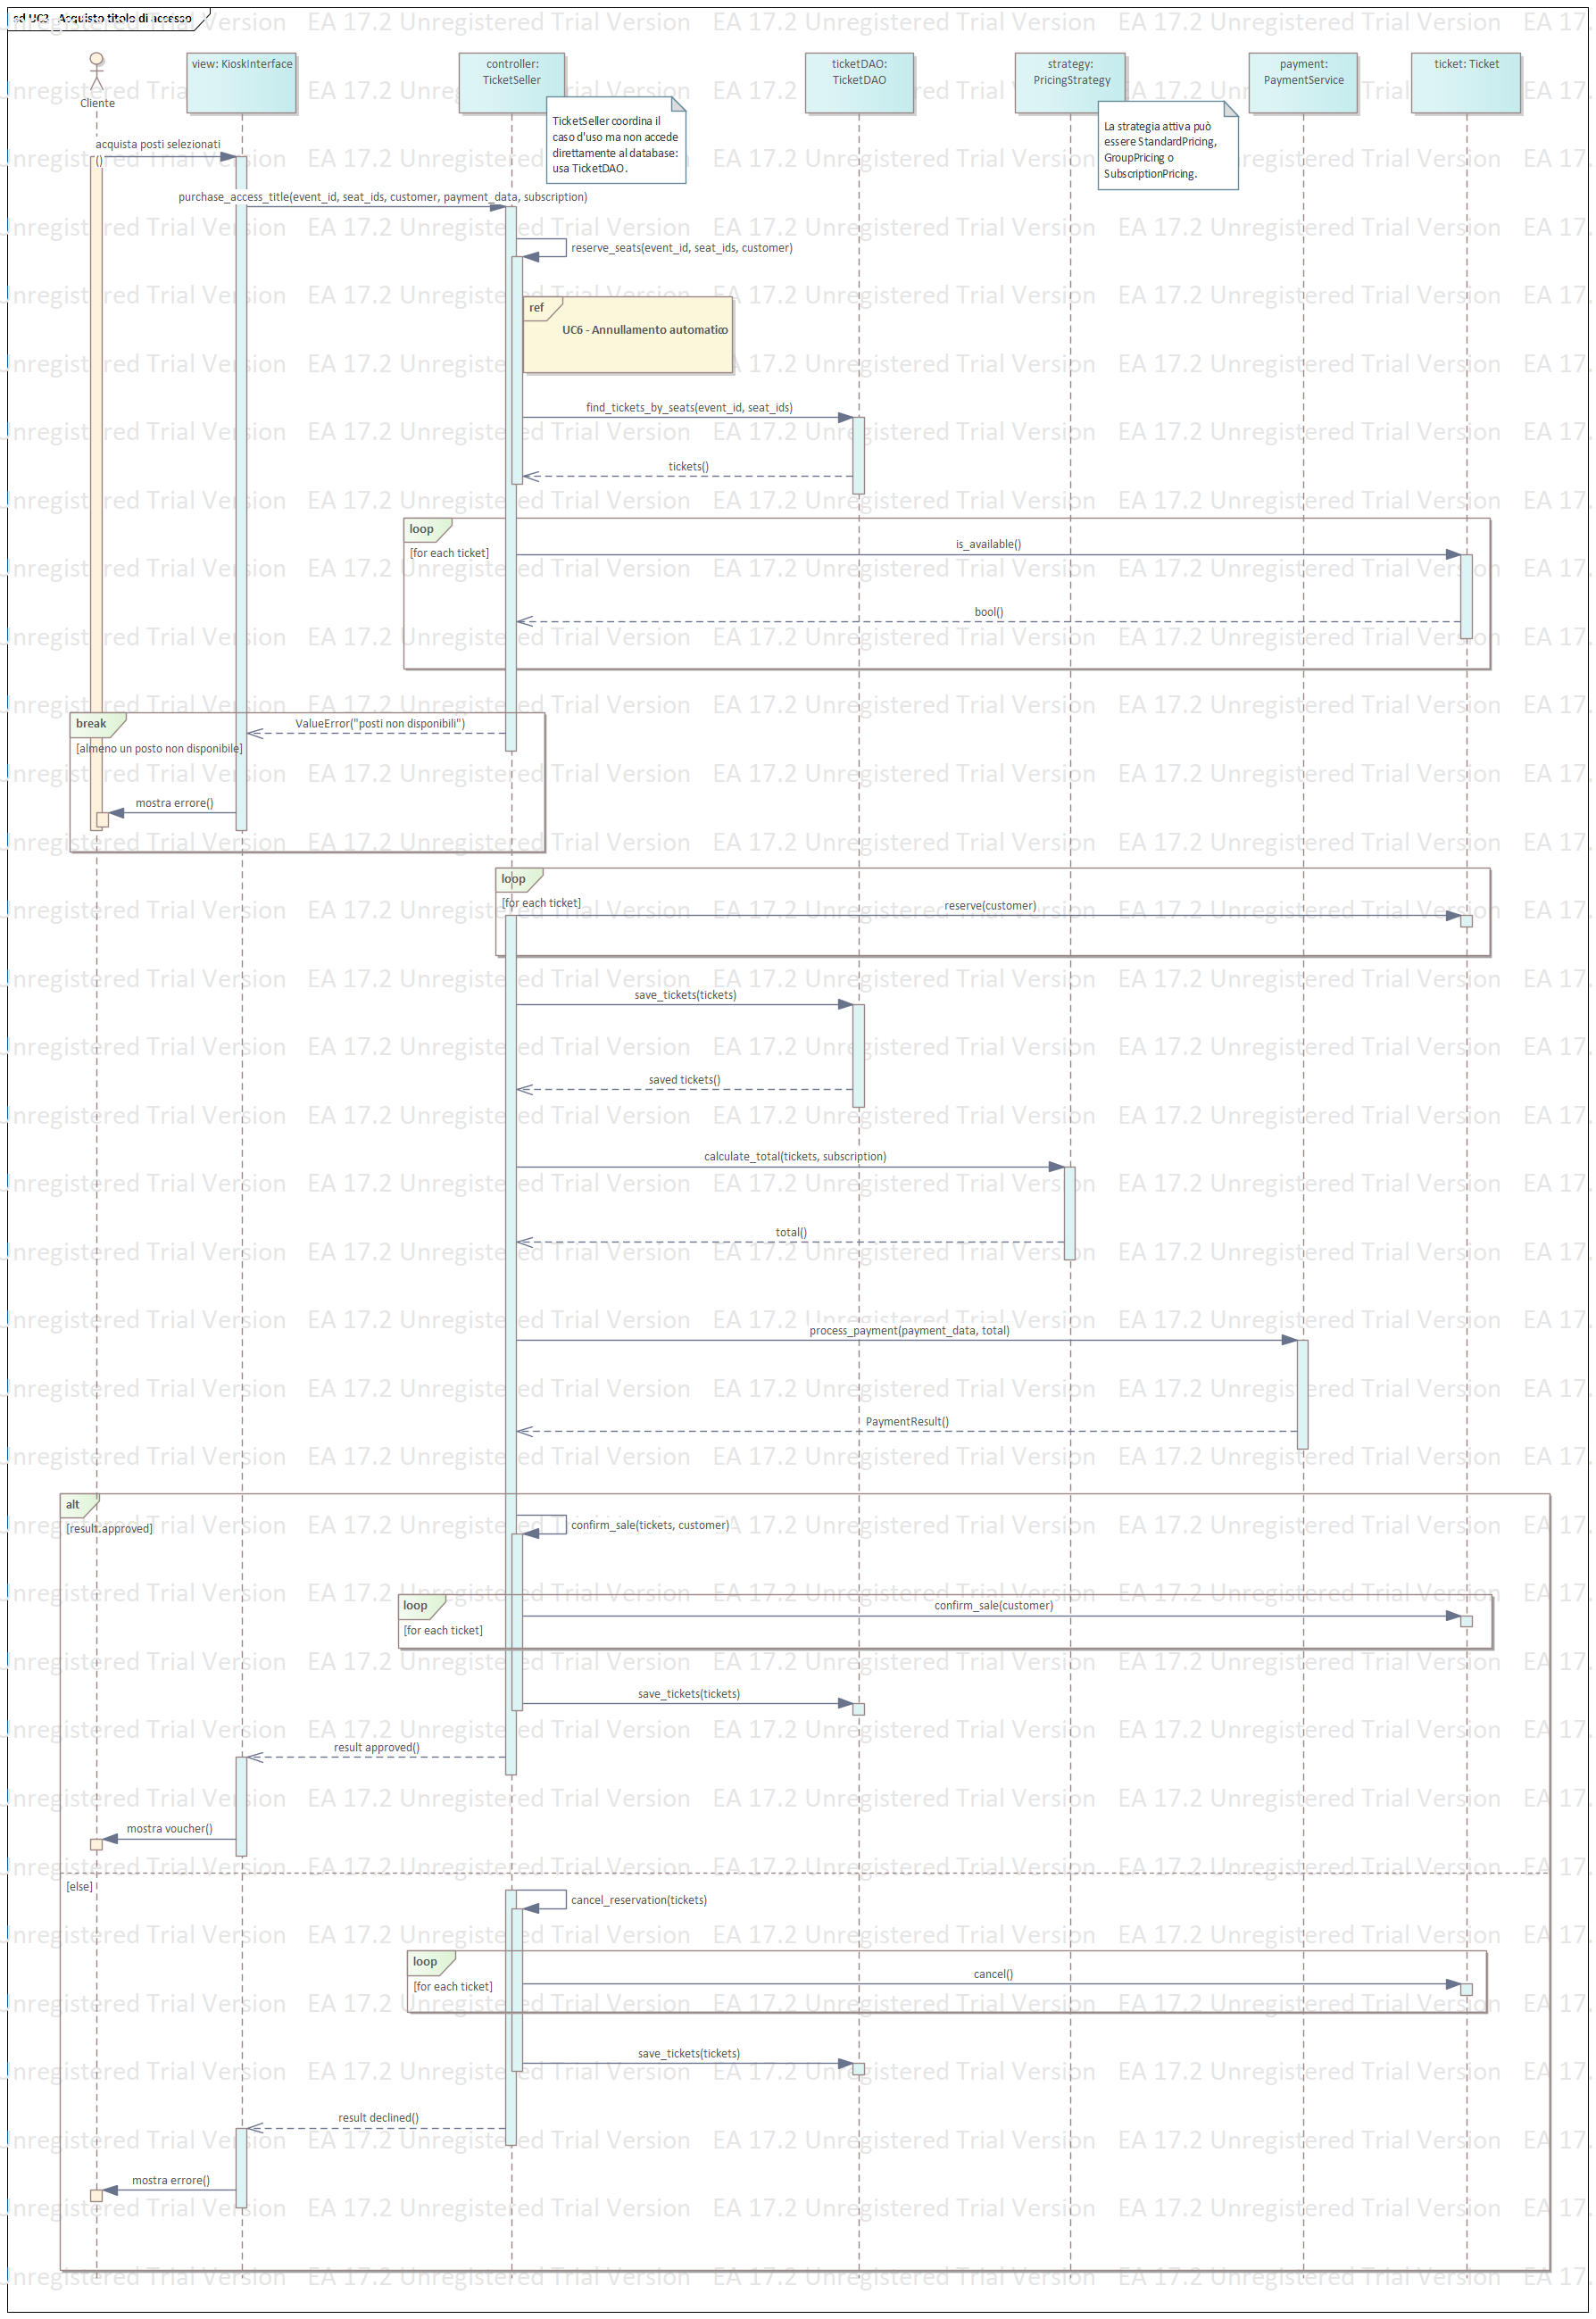
\includegraphics[height=0.88\textheight,width=\textwidth,keepaspectratio]{UC3_-_Acquisto_titolo_di_accesso.png}
\caption{Sequenza UC3 -- Acquisto titolo di accesso}
\label{fig:sd3}
\end{figure}
Il controller esegue \code{reserve_seats}: dopo l'annullamento delle prenotazioni scadute legge i biglietti e ne verifica la disponibilità. Se almeno un posto non è disponibile l'interazione termina con un errore (frammento \texttt{break}); altrimenti i biglietti sono bloccati e salvati, il totale è calcolato dalla strategia di prezzo e il pagamento è inviato al servizio esterno. Il frammento \texttt{alt} distingue il pagamento approvato (\code{confirm_sale} e codice della transazione) da quello rifiutato (\code{cancel_reservation} e messaggio di errore).

\subsubsection{UC4 -- Utilizzo abbonamento}
\diagramma[0.8\textwidth]{UC4_-_Utilizzo_abbonamento.png}{Sequenza UC4 -- Utilizzo abbonamento}{fig:sd4}
Il cliente inserisce il codice; la vista ottiene l'abbonamento con \code{find_subscription}. Quando l'abbonamento è presente il controller usa la strategia \code{SubscriptionPricing}, che sconta i biglietti degli eventi coperti.

\subsubsection{UC5 -- Gestione catalogo eventi}
\begin{figure}[H]
\centering
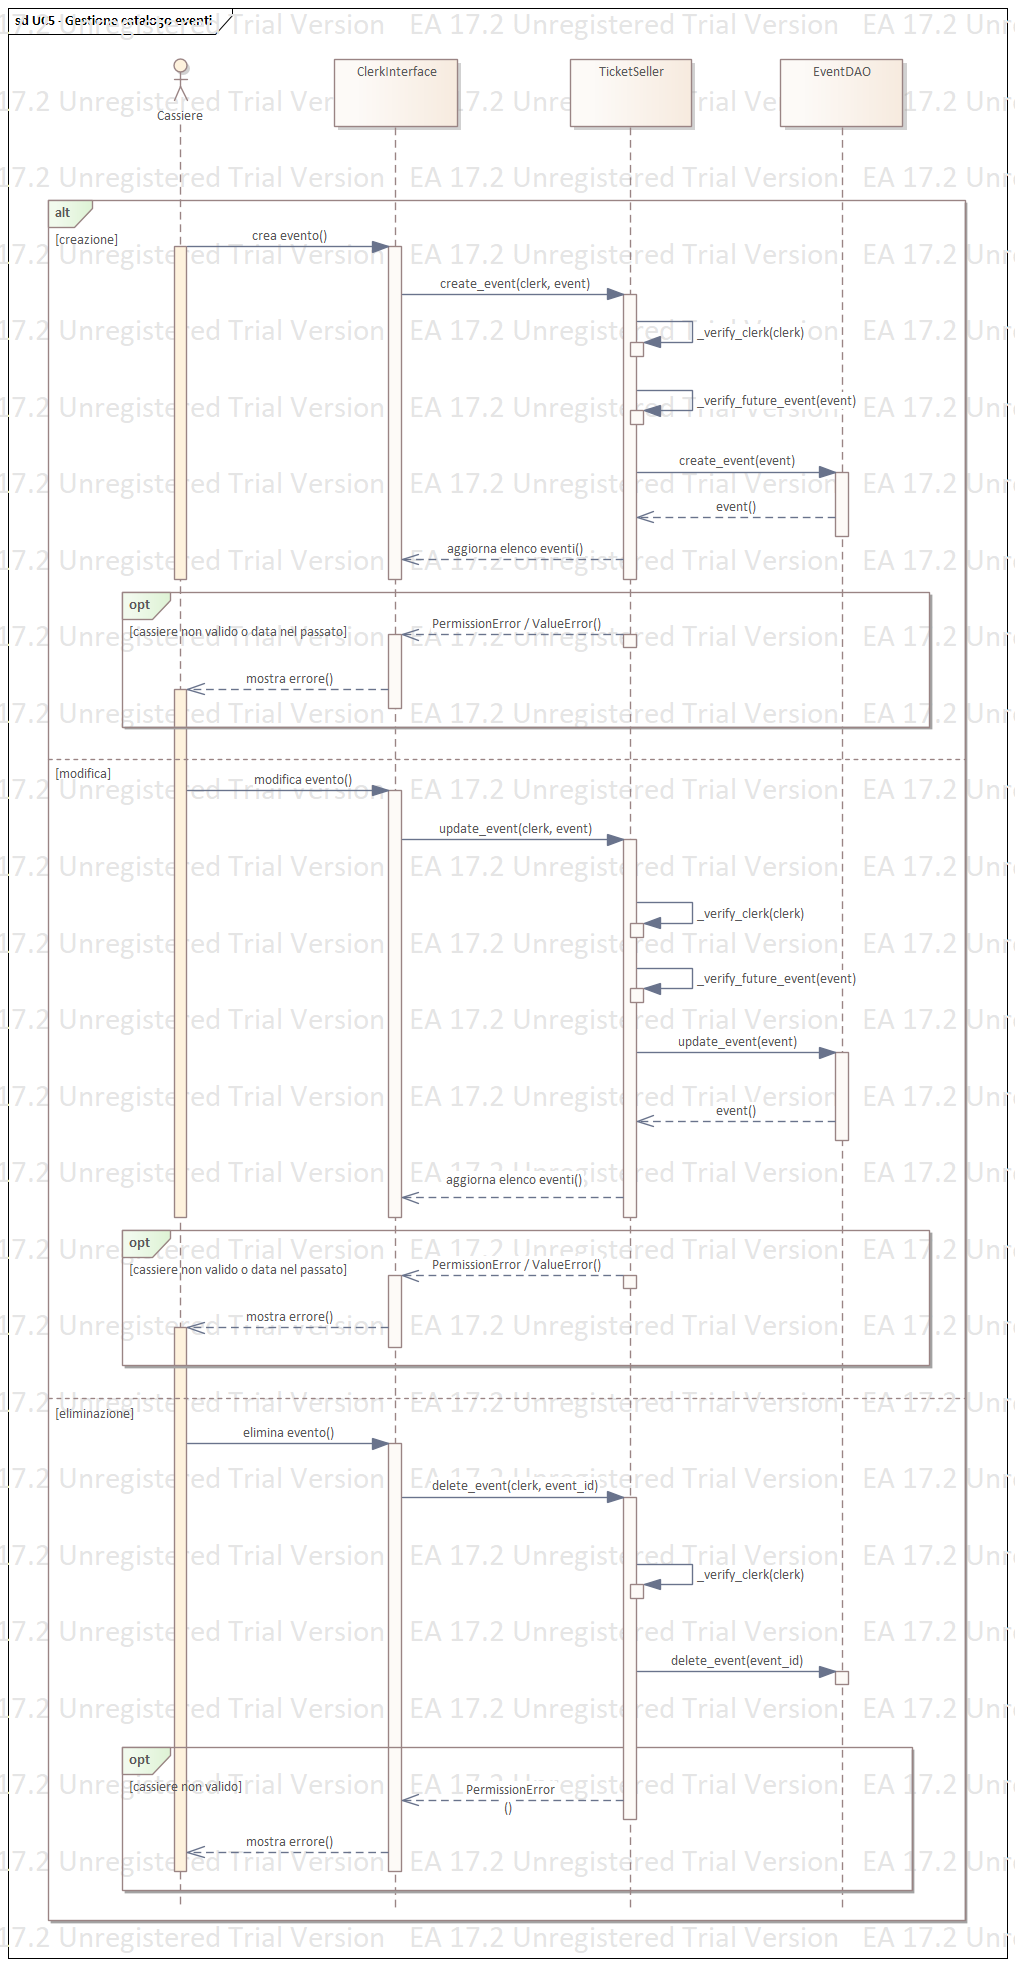
\includegraphics[height=0.88\textheight,width=\textwidth,keepaspectratio]{UC5_-_Gestione_catalogo_eventi.png}
\caption{Sequenza UC5 -- Gestione catalogo eventi}
\label{fig:sd5}
\end{figure}
Il frammento \texttt{alt} separa creazione, modifica ed eliminazione. In ogni ramo il controller verifica il cassiere (\code{_verify_clerk}) e, per creazione e modifica, la data futura (\code{_verify_future_event}), poi delega al DAO. Il frammento \texttt{opt} di ciascun ramo mostra il caso in cui un controllo non è superato: l'eccezione torna alla vista, che mostra l'errore.

\subsubsection{UC6 -- Annullamento automatico}
\diagramma[0.75\textwidth]{UC6_-_Annullamento_automatico.png}{Sequenza UC6 -- Annullamento automatico}{fig:sd6}
L'attore Tempo avvia \code{release_expired_reservations}: il controller legge i biglietti, annulla quelli bloccati da almeno 15 minuti e, se ce ne sono, li salva.

\subsection{Diagrammi di attività}
\label{sec:attivita}

Per ogni scenario si riporta un diagramma di attività con partizioni (chi esegue l'azione), nodi di decisione con guardie e nodi iniziale e finale.

\subsubsection{UC1 -- Consultazione eventi}
\diagramma[0.62\textwidth]{ACT_-_UC1_Consultazione_eventi.png}{Attività UC1 -- Consultazione eventi}{fig:act1}

\subsubsection{UC2 -- Selezione posti}
\diagramma[0.68\textwidth]{ACT_-_UC2_Selezione_posti.png}{Attività UC2 -- Selezione posti}{fig:act2}

\subsubsection{UC3 -- Acquisto titolo di accesso}
\diagramma{ACT_-_UC3_Acquisto_titolo_di_accesso.png}{Attività UC3 -- Acquisto titolo di accesso}{fig:act3}
Il cliente sceglie evento e posti, vede il totale, inserisce i dati di pagamento e conferma. Il sistema rilascia le prenotazioni scadute e controlla la disponibilità: se un posto non è disponibile mostra un errore, altrimenti blocca i posti, calcola il totale e invia il pagamento. In base all'esito conferma la vendita o annulla il blocco; in entrambi i casi salva i biglietti e mostra il risultato.

\subsubsection{UC4 -- Utilizzo abbonamento}
\diagramma[0.62\textwidth]{ACT_-_UC4_Utilizzo_abbonamento.png}{Attività UC4 -- Utilizzo abbonamento}{fig:act4}

\subsubsection{UC5 -- Gestione catalogo eventi}
\diagramma{ACT_-_UC5_Gestione_catalogo_eventi.png}{Attività UC5 -- Gestione catalogo eventi}{fig:act5}
Dopo la scelta dell'operazione il controller verifica il cassiere e, per creazione e modifica, la data dell'evento; se un controllo fallisce il flusso confluisce nel ramo di errore, altrimenti il DAO esegue l'operazione e la vista aggiorna l'elenco.

\subsubsection{UC6 -- Annullamento automatico}
\diagramma[0.85\textwidth]{ACT_-_UC6_Annullamento_automatico.png}{Attività UC6 -- Annullamento automatico}{fig:act6}
Il ciclo esamina un biglietto alla volta: se è bloccato e il blocco dura da almeno 15 minuti lo annulla e lo aggiunge alla lista dei rilasciati. Finiti i biglietti, la lista viene salvata solo se non è vuota.

\section{Progettazione}
\label{sec:progettazione}

\subsection{Architettura}

TicketSeller segue il pattern architetturale \textbf{Model--View--Controller}, con uno strato \textbf{DAO} per l'accesso ai dati.

\begin{tabularx}{\textwidth}{@{}L{2.9cm}Y@{}}
\toprule
\textbf{Strato} & \textbf{Responsabilità} \\
\midrule
View & \code{KioskInterface} e \code{ClerkInterface} (PyQt6): ricevono l'input, lo passano al controller e mostrano risultati ed errori. \\
Controller & \code{TicketSeller}: coordina i casi d'uso, applica le regole applicative (blocco dei posti, timeout, controllo del cassiere) e usa DAO, strategie di prezzo e servizio di pagamento. \\
Model & Entità \code{Event}, \code{Voucher}, \code{Ticket}, \code{Subscription}, \code{User}, \code{Customer}, \code{Clerk}; stati del biglietto (State) e politiche di prezzo (Strategy). \\
DAO & Interfacce \code{EventDAO}, \code{TicketDAO}, \code{SubscriptionDAO}; implementazione \code{TicketDB} su file JSON. \\
Servizi esterni & \code{CreditCardCharges}, adattatore (simulato) verso il servizio di pagamento, conforme a \code{PaymentService}. \\
\bottomrule
\end{tabularx}

Le scelte seguono i principi di progettazione del corso:

\begin{itemize}
    \item \textbf{coesione}: ogni package ha responsabilità omogenee (vista, controllo, dominio, persistenza, pagamento);
    \item \textbf{basso accoppiamento e astrazione}: il controller dipende dalle interfacce \code{EventDAO}, \code{TicketDAO}, \code{SubscriptionDAO}, \code{PricingStrategy} e \code{PaymentService} e riceve le implementazioni nel costruttore (le crea \code{app.py});
    \item \textbf{incapsulamento}: le regole sulle transizioni del biglietto stanno negli oggetti stato, non nel controller;
    \item \textbf{flessibilità}: una nuova politica di prezzo si aggiunge con una nuova strategia, senza modificare il controller;
    \item \textbf{testabilità}: la logica non dipende dalla GUI e il pagamento può essere sostituito da uno stub nei test;
    \item \textbf{progettazione difensiva}: i dati sono validati ai confini (costruttori dei modelli, dati della carta, controller) e gli errori sono segnalati con eccezioni mostrate dalla vista.
\end{itemize}

Rispetto alla forma classica del pattern MVC, in cui il model notifica le viste a ogni modifica, in TicketSeller è la vista che, dopo ogni operazione, richiede i dati aggiornati al controller.

\subsection{Classi di progettazione}

\diagramma[0.72\textwidth]{CLS_-_Classi_di_progettazione.png}{Package di progettazione e dipendenze}{fig:cls}

I package corrispondono alle cartelle di \code{src/ticketseller}: \code{views}, \code{controllers}, \code{models}, \code{dao}, \code{patterns} (\code{state} e \code{strategy}) ed \code{external_services}. Le classi indicate come interfacce sono, in Python, classi astratte (\code{ABC} con metodi \code{@abstractmethod}); \code{PaymentService} è un \code{Protocol}, realizzato da \code{CreditCardCharges}.

\subsubsection*{Package controllers}
\diagramma{controllers.png}{Classi di progettazione: controllers}{fig:cls-controllers}
\code{TicketSeller} è l'unico controller. Riceve nel costruttore i DAO, il servizio di pagamento, la strategia di prezzo normale e quella per gli abbonamenti; \code{_reservation_lock} protegge le operazioni sui posti.

\subsubsection*{Package models}
\diagramma[0.9\textwidth]{models.png}{Classi di progettazione: models}{fig:cls-models}
\code{Ticket} è il contesto del pattern State: il suo attributo \code{state} punta allo stato corrente.

\subsubsection*{Package dao}
\diagramma{dao.png}{Classi di progettazione: dao}{fig:cls-dao}
\code{TicketDB} realizza le tre interfacce DAO e nasconde il formato di memorizzazione (file JSON): per passare a un database basta un'altra classe che realizza le stesse interfacce.

\subsubsection*{Package patterns}
\diagramma[0.85\textwidth]{state.png}{Classi di progettazione: pattern State}{fig:cls-state}
\diagramma{strategy.png}{Classi di progettazione: pattern Strategy}{fig:cls-strategy}

\subsubsection*{Package external\_services}
\diagramma[0.85\textwidth]{external_services.png}{Classi di progettazione: external\_services}{fig:cls-ext}

\subsubsection*{Package views}
\diagramma[0.75\textwidth]{views.png}{Classi di progettazione: views}{fig:cls-views}
Le due viste ereditano da \code{QWidget} e conoscono solo il controller.

\subsection{Diagramma dei componenti}

\diagramma[0.9\textwidth]{CMP_-_Componenti_TicketSeller.png}{Diagramma dei componenti}{fig:cmp}

Le viste usano l'interfaccia del controller \code{TicketSeller}, che a sua volta richiede le interfacce \code{TicketDAO}, \code{SubscriptionDAO}, \code{EventDAO} (fornite dal componente DAO, realizzato da \code{TicketDB}), \code{PricingStrategy} (fornita dalle strategie) e \code{PaymentService} (fornita da \code{CreditCardCharges}). Il componente \code{Models} richiede l'interfaccia \code{TicketState}, fornita dagli stati.

\subsection{Macchina a stati del biglietto}

\diagramma[0.85\textwidth]{STM_-_Stato_Ticket.png}{Macchina a stati del biglietto}{fig:stm}

\begin{tabularx}{\textwidth}{@{}L{1.9cm}L{1.9cm}Y@{}}
\toprule
\textbf{Da} & \textbf{A} & \textbf{Evento [guardia] / azione} \\
\midrule
(iniziale) & Available & creazione del biglietto con l'evento \\
Available & Locked & \code{reserve(customer)} \\
Locked & Available & \code{cancel} [pagamento rifiutato o errore nel pagamento] \\
Locked & Available & quando now $-$ \code{locked_at} $\geq$ 15 min / \code{cancel()} \\
Locked & Sold & \code{confirm_sale(customer)} \\
Available, Locked & (finale) & \code{delete_event} \\
Sold & (finale) & fine del processo di vendita \\
\bottomrule
\end{tabularx}

Le operazioni non ammesse nello stato corrente (ad esempio \code{confirm_sale} su un biglietto disponibile, o qualsiasi operazione su un biglietto venduto) sollevano un errore e lasciano il biglietto nello stato in cui si trova.

\subsection{Diagramma di deployment}

\diagramma[0.9\textwidth]{DEP_-_Deployment_TicketSeller.png}{Diagramma di deployment}{fig:dep}

L'applicazione è un programma desktop. Ogni postazione (PC Windows, macOS o Linux) esegue in un interprete Python~3.11+ con PyQt6 lo stesso artefatto \code{ticketseller}, avviato in modalità kiosk o cassiere, che legge e scrive il file \code{database.json}. Si assume che sull'archivio lavori una postazione alla volta. L'artefatto manifesta i componenti \code{KioskInterface}, \code{ClerkInterface}, \code{TicketSeller} e \code{TicketDB}. L'agenzia delle carte di credito è un sistema esterno, simulato nel prototipo.

\section{Mockup}
\label{sec:mockup}

Le schermate seguenti sono le interfacce realizzate con PyQt6.

\diagramma[0.72\textwidth]{kiosk.png}{Interfaccia del kiosk (cliente)}{fig:kiosk}

In alto il cliente sceglie l'evento (UC1); sotto compare la mappa dei posti con codice, stato e prezzo, dove i posti bloccati o venduti non sono selezionabili (UC2). Il totale si aggiorna a ogni selezione e tiene conto dell'eventuale codice abbonamento (UC4): nell'esempio due posti da 30,00 con l'abbonamento al 50\% danno 30,00. Nel riquadro \emph{Payment} il cliente inserisce i suoi dati e quelli della carta; \emph{Buy Selected Seats} avvia l'acquisto (UC3) e l'esito è mostrato in una finestra di dialogo. \emph{Refresh} ricarica gli eventi.

\diagramma[0.72\textwidth]{clerk.png}{Interfaccia del cassiere}{fig:clerk}

La postazione del cassiere mostra gli eventi futuri; selezionandone uno il modulo si compila con i suoi dati. I pulsanti \emph{Create}, \emph{Update} e \emph{Delete} eseguono le operazioni di UC5 e gli eventuali errori di validazione sono mostrati in una finestra di dialogo.

\section{Implementazione}
\label{sec:implementazione}

\subsection{Tecnologie e struttura}

Il programma è scritto in \textbf{Python 3.11+} con interfaccia grafica \textbf{PyQt6}. Le entità sono \code{dataclass}, le interfacce sono classi astratte (\code{abc}), gli importi usano \code{Decimal} per evitare errori di arrotondamento e i dati sono salvati in un file JSON. I test usano \code{unittest} (PyUnit); i diagrammi sono stati fatti con Enterprise Architect.

Il codice è in \code{src/ticketseller}, con una cartella per ogni parte (\code{views}, \code{controllers}, \code{models}, \code{dao}, \code{patterns}, \code{external_services}). Il file \code{app.py} crea gli oggetti, li passa al controller e apre la finestra richiesta:

\par\noindent\begin{minipage}{\linewidth}
\begin{lstlisting}
python -m ticketseller.app kiosk     # postazione del cliente
python -m ticketseller.app clerk     # postazione del cassiere
\end{lstlisting}
\end{minipage}\par

Negli estratti seguenti sono stati tolti commenti, docstring e alcune annotazioni di tipo.

\subsection{Controller}

Il controller riceve dall'esterno tutto quello che usa (DAO, servizio di pagamento, strategie di prezzo): così nei test si possono passare oggetti di prova.

\par\noindent\begin{minipage}{\linewidth}
\begin{lstlisting}
class TicketSeller:
    reservation_timeout = timedelta(minutes=15)

    def __init__(self, event_dao, ticket_dao, payment_service, pricing_strategy,
                 subscription_strategy=None, subscription_dao=None):
        self.event_dao = event_dao
        self.ticket_dao = ticket_dao
        self.payment_service = payment_service
        self.pricing_strategy = pricing_strategy
        self.subscription_strategy = subscription_strategy
        self.subscription_dao = subscription_dao
        self._reservation_lock = RLock()
\end{lstlisting}
\end{minipage}\par

\subsection{Acquisto}

\code{purchase_access_title} esegue l'acquisto (UC3): blocca i posti, calcola il totale, chiede il pagamento e poi conferma la vendita o libera i posti. Se i dati della carta non sono validi il pagamento solleva un errore: prima di passarlo alla finestra, i posti vengono liberati.

\par\noindent\begin{minipage}{\linewidth}
\begin{lstlisting}
def purchase_access_title(self, event_id, seat_ids, customer, payment_data, subscription=None):
    tickets = self.reserve_seats(event_id, seat_ids, customer)
    try:
        total = self.calculate_total(tickets, subscription)
        result = self.payment_service.process_payment(payment_data, total)
    except ValueError:
        self.cancel_reservation(tickets)
        raise
    if result.approved:
        self.confirm_sale(tickets, customer)
    else:
        self.cancel_reservation(tickets)
    return result
\end{lstlisting}
\end{minipage}\par

In \code{reserve_seats} il controllo dei posti e il blocco avvengono sotto un lock, così due richieste contemporanee non possono prendere lo stesso posto (RNF3):

\par\noindent\begin{minipage}{\linewidth}
\begin{lstlisting}
def reserve_seats(self, event_id, seat_ids, customer=None):
    with self._reservation_lock:
        self.release_expired_reservations(event_id)
        if len({str(seat_id) for seat_id in seat_ids}) != len(seat_ids):
            raise ValueError("Duplicate seats cannot be selected.")
        tickets = self.ticket_dao.find_tickets_by_seats(event_id, seat_ids)
        if not tickets:
            raise ValueError("At least one seat must be selected.")
        if any(not ticket.is_available() for ticket in tickets):
            raise ValueError("One or more selected seats are not available.")
        for ticket in tickets:
            ticket.reserve(customer)
        return self.ticket_dao.save_tickets(tickets)
\end{lstlisting}
\end{minipage}\par

\subsection{Pattern State}

Il biglietto non decide da solo cosa fare: passa la richiesta al suo stato corrente, che controlla se l'operazione è permessa e cambia stato.

\par\noindent\begin{minipage}{\linewidth}
\begin{lstlisting}
class Ticket(Voucher):
    def reserve(self, customer=None):
        self.state.reserve(self, customer)

    def cancel(self):
        self.state.cancel(self)

    def confirm_sale(self, customer):
        self.state.confirm_sale(self, customer)


class LockedState(TicketState):
    def reserve(self, ticket, customer=None):
        raise ValueError("Ticket is already locked.")

    def cancel(self, ticket):
        ticket.set_state(AvailableState())
        ticket.locked_at = None
        ticket.owner = None

    def confirm_sale(self, ticket, customer):
        if ticket.owner is not None and ticket.owner != customer:
            raise ValueError("Ticket is locked by another customer.")
        ticket.set_state(SoldState())
        ticket.locked_at = None
        ticket.owner = customer
\end{lstlisting}
\end{minipage}\par

\subsection{Pattern Strategy}

Ogni politica di prezzo è una classe con il metodo \code{calculate_total}. Il controller usa la strategia per gli abbonamenti quando il cliente ne indica uno, altrimenti quella normale.

\par\noindent\begin{minipage}{\linewidth}
\begin{lstlisting}
def calculate_total(self, tickets, subscription=None):
    strategy = self.pricing_strategy
    if subscription is not None and self.subscription_strategy is not None:
        strategy = self.subscription_strategy
    return strategy.calculate_total(tickets, subscription)


class SubscriptionPricing(PricingStrategy):
    def calculate_total(self, tickets, subscription=None):
        if subscription is None:
            raise ValueError("Subscription pricing requires a subscription.")
        discount_rate = subscription.discount_rate if subscription.discount_rate is not None else Decimal("1.00")
        total = Decimal("0.00")
        for ticket in tickets:
            if ticket.event_id in subscription.covered_event_ids:
                total += ticket.base_price * (Decimal("1.00") - discount_rate)
            else:
                total += ticket.base_price
        return quantize_money(total)
\end{lstlisting}
\end{minipage}\par

\subsection{Persistenza e rilascio dei posti}

\code{TicketDB} tiene i dati in memoria e a ogni modifica riscrive il file \code{database.json}; all'avvio lo rilegge. Il resto del programma non sa che i dati stanno in un file, perché usa solo le interfacce DAO: per passare a un database basterebbe un'altra classe che le realizza.

Il kiosk avvia un timer che ogni minuto libera i posti bloccati da più di 15 minuti (attore Tempo, UC6):

\par\noindent\begin{minipage}{\linewidth}
\begin{lstlisting}
self.release_timer = QTimer(self)
self.release_timer.timeout.connect(self._release_expired_reservations)
self.release_timer.start(60_000)
\end{lstlisting}
\end{minipage}\par

\section{Test}
\label{sec:test}

\subsection{Come sono fatti i test}

I test sono scritti con \code{unittest} (PyUnit), si trovano nella cartella \code{tests} e si eseguono con

\par\noindent\begin{minipage}{\linewidth}
\begin{lstlisting}
python -m unittest discover -s tests -v
\end{lstlisting}
\end{minipage}\par

Sono \textbf{65 test} e passano tutti.

Ogni test parte da dati nuovi, creati nel metodo \code{setUp}, quindi i test non dipendono l'uno dall'altro. Stati, strategie di prezzo e modelli sono provati da soli (test di unità). Il controller è provato insieme al DAO tenuto in memoria, senza file (test di integrazione); al posto del servizio di pagamento vero si usa un oggetto di prova, \code{FixedPaymentService}, che risponde sempre allo stesso modo (\emph{stub}). I casi sono scelti a partire dai requisiti, provando sia i dati giusti sia quelli sbagliati (posti liberi, bloccati, venduti, inesistenti; carte valide e scadute) e i valori al limite (timeout appena sotto e appena sopra i 15 minuti, sconto dello 0\% e del 100\%).

{\small
\begin{tabularx}{\textwidth}{@{}L{6.0cm}Y@{}}
\toprule
\textbf{File} & \textbf{Cosa verifica} \\
\midrule
\code{test_ticket_state.py} & Passaggi di stato del biglietto e operazioni non permesse. \\
\code{test_pricing_strategy.py} & Prezzo normale, sconto di gruppo, abbonamento, arrotondamento al centesimo. \\
\code{test_ticket_seller_controller.py} & Acquisto approvato e rifiutato, posti duplicati, timeout, gestione degli eventi. \\
\code{test_requirements.py} & Un test per ogni requisito e i casi corretti durante lo sviluppo. \\
\code{test_subscription.py} & Ricerca dell'abbonamento per codice e acquisto scontato. \\
\code{test_ticket_db.py} & Salvataggio e lettura dal file, mappa dei posti, vincoli sugli eventi. \\
\code{test_payment_service.py}, \code{test_model_validation.py}, \code{test_utils.py} & Controllo dei dati della carta, dei modelli e delle date. \\
\bottomrule
\end{tabularx}}

\subsection{Esempi}

Pagamento approvato: il biglietto risulta venduto.

\par\noindent\begin{minipage}{\linewidth}
\begin{lstlisting}
def test_successful_purchase_sells_ticket(self) -> None:
    controller = TicketSeller(self.db, self.db, FixedPaymentService(True), StandardPricing())
    result = controller.purchase_access_title(EventId(1), [SeatId("S001")], self.customer, self.payment)
    ticket = self.db.find_tickets_by_seats(EventId(1), [SeatId("S001")])[0]
    self.assertTrue(result.approved)
    self.assertEqual("sold", ticket.state.name())
\end{lstlisting}
\end{minipage}\par

Carta non valida: viene segnalato l'errore e il posto torna disponibile.

\par\noindent\begin{minipage}{\linewidth}
\begin{lstlisting}
def test_rf8_invalid_card_releases_reserved_seats(self) -> None:
    controller = TicketSeller(self.db, self.db, CreditCardCharges(success_rate=1.0), StandardPricing())
    bad_card = PaymentData("Alice Buyer", "not-a-card", 12, 2099, "123")
    with self.assertRaises(ValueError):
        controller.purchase_access_title(EventId(1), [SeatId("S001")], self.customer, bad_card)
    self.assertEqual("available", self._ticket("S001").state.name())
\end{lstlisting}
\end{minipage}\par

\subsection{Requisiti e test}

\small
\begin{center}
\begin{tabular}{@{}L{1.8cm}L{12.3cm}@{}}
\toprule
\textbf{Requisito} & \textbf{Test principale} \\
\midrule
RF1 & \code{test_rf1_search_future_events_excludes_past_events} \\
RF2 & \code{test_rf2_seating_map_lists_every_seat_with_state} \\
RF3 & \code{test_rf3_check_availability_reports_locked_seats}, \code{test_rf4_reserve_locks_seats_for_customer} \\
RF4 & \code{test_invalid_card_number_is_rejected} \\
RF5 & \code{test_rf5_runtime_strategy_change_applies_group_discount} \\
RF6 & \code{test_rf6_payment_service_receives_computed_total} \\
RF7 & \code{test_successful_purchase_sells_ticket} \\
RF8 & \code{test_declined_purchase_releases_ticket}, \code{test_rf8_invalid_card_releases_reserved_seats} \\
RF9, RNF7 & \code{test_rf9_rnf7_timeout_boundary} \\
RF10 & \code{test_rf10_clerk_creates_event_with_seating_map} \\
RF11 & \code{test_rf11_clerk_updates_event} \\
RF12 & \code{test_rf12_clerk_deletes_event}, \code{test_delete_event_with_reserved_ticket_is_rejected} \\
RF13 & \code{test_rf13_subscription_purchase_charges_discounted_amount} \\
RNF3 & \code{test_rnf3_concurrent_reservations_allow_one_winner} \\
RNF4 & \code{test_money_is_rounded_half_up} \\
RNF5 & \code{test_rnf5_json_roundtrip_preserves_states_owner_and_lock_time} \\
\bottomrule
\end{tabular}
\end{center}
\normalsize

\section*{Conclusioni}
\addcontentsline{toc}{section}{Conclusioni}

Il progetto segue tutte le fasi viste nel corso, dai requisiti ai test. L'architettura MVC tiene separate le finestre, la logica e i dati; il DAO nasconde il modo in cui i dati sono salvati; i pattern State e Strategy rendono chiare le regole sui biglietti e sui prezzi.

Il prototipo ha alcuni limiti: il pagamento è simulato, il cassiere non deve autenticarsi e si assume che sull'archivio lavori una postazione alla volta. Per usarlo con più postazioni basterebbe sostituire il file con un database, cambiando solo la classe \code{TicketDB}.


\end{document}
